\documentclass[10pt,compress]{beamer}
\usepackage[utf8]{inputenc}          % UTF-8 Encoding
\usepackage{hyperref}                % Interactive PDF

% Layout
\useinnertheme[sectionpage=none]{metropolis}
\useoutertheme[numbering=fraction]{metropolis}
\usetheme[everytitleformat=regular]{m}
\metroset{block=fill}

%% Hide navigation buttons
\beamertemplatenavigationsymbolsempty

%% Meta-stuff like authors, title, etc.
\author[Daniel Hillerström]{Daniel Hillerström\\\footnotesize{\href{mailto:daniel.hillerstrom@ed.ac.uk}{daniel.hillerstrom@ed.ac.uk}}\\\footnotesize{\href{http://homepages.inf.ed.ac.uk/s1467124}{http://homepages.inf.ed.ac.uk/s1467124}}}
\institute[University of Edinburgh]{CDT Pervasive Parallelism, University of Edinburgh}
\date{\today}
\title{Effective Concurrency} % Just some title; change at a later point.
\subtitle{Pervasive Parallelism Presentation}

% The document
\begin{document}
  \maketitle
  % Input the content

  \begin{frame}
    \frametitle{Different concurrent programming models}
    \textbf{Message-passing programming (distributed memory)}
    \begin{itemize}
      \item MPI
      \item Erlang
    \end{itemize}
    \textbf{Multi-threaded programming (shared memory)}
    \begin{itemize}
      \item OpenMP
      \item Java
    \end{itemize}
    \textbf{Partition Global Address Space programming (hybrid)}
    \begin{itemize}
      \item Coarray Fortran
      \item Unified Parallel C
    \end{itemize}
  \end{frame}

  \begin{frame}
    \frametitle{Combining concurrency models}
    Different concurrency models are tailored for particular idioms
    \begin{description}
      \item[\alert<1->{MPI}] Process-centric; interaction among processes across many machines.
      \item[\alert<1->{OpenMP}] Thread-centric; interaction between cores on a chip.
    \end{description}
    Sometimes it makes sense to combine different concurrency models.
  \end{frame}

  % Slide 3
  \begin{frame}
    \frametitle{Commonalities}
    \begin{center}
      \begin{figure}
        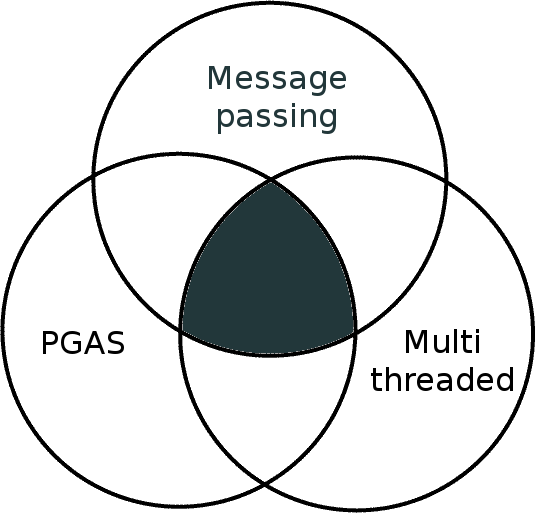
\includegraphics[scale=0.3]{venn.png}
      \end{figure}
    \end{center}
    \uncover<2->{What is the proper abstraction?}
  \end{frame}

  % Aims and objectives
  \begin{frame}
    \frametitle{Aims and objectives}
    The aim is to implement an optimizing compiler for Links.
    \begin{itemize}
       \item Efficient implementation of handlers.
       \item Concurrency for ``free'' through handlers.
    \end{itemize}
  \end{frame}

  % Evaluation
  \begin{frame}
    \frametitle{Evaluation}
    Collection of micro-benchmarks
    \begin{itemize}
      \item Sanity checks
      \item Already written
    \end{itemize}
    Collection of performance benchmarks
    \begin{itemize}
      \item Measuring the feasibility of my implementation
      \item Building the benchmark suite from PLDI\dots
    \end{itemize}
  \end{frame}
\end{document}